%%%%%%%%%%%%%%%%%%%%%%%%%%%%%%%%%%%%%%%%%%%%%%%%%%%%%%%%%%%%%%%%%%%%%%%%%%%%%%%

\section*{\large Exercício 1 - Simulação de Sinais Estocásticos com GRNG1.py com N valores de medidas}
\addcontentsline{toc}{chapter}{\protect\numberline{}\large Exercício 1}%

Os resultados das análises dos sinais referentes a este exercício se encontram na pasta \textbf{Exercise1}. Abaixo está um plot com dez sinais para a série com $N$ = 64 da família noise, junto com seus respectivos histogramas.

% EXEMPLO PARA ADICIONAR FIGURA
\begin{figure}[ht!]
	%\caption{Série e histogramas.}
	\vspace{0mm}	% acrescentar o espaçamento vertical apropriado entre o título e a borda superior da figura
	\begin{center}
		\resizebox{15cm}{!}{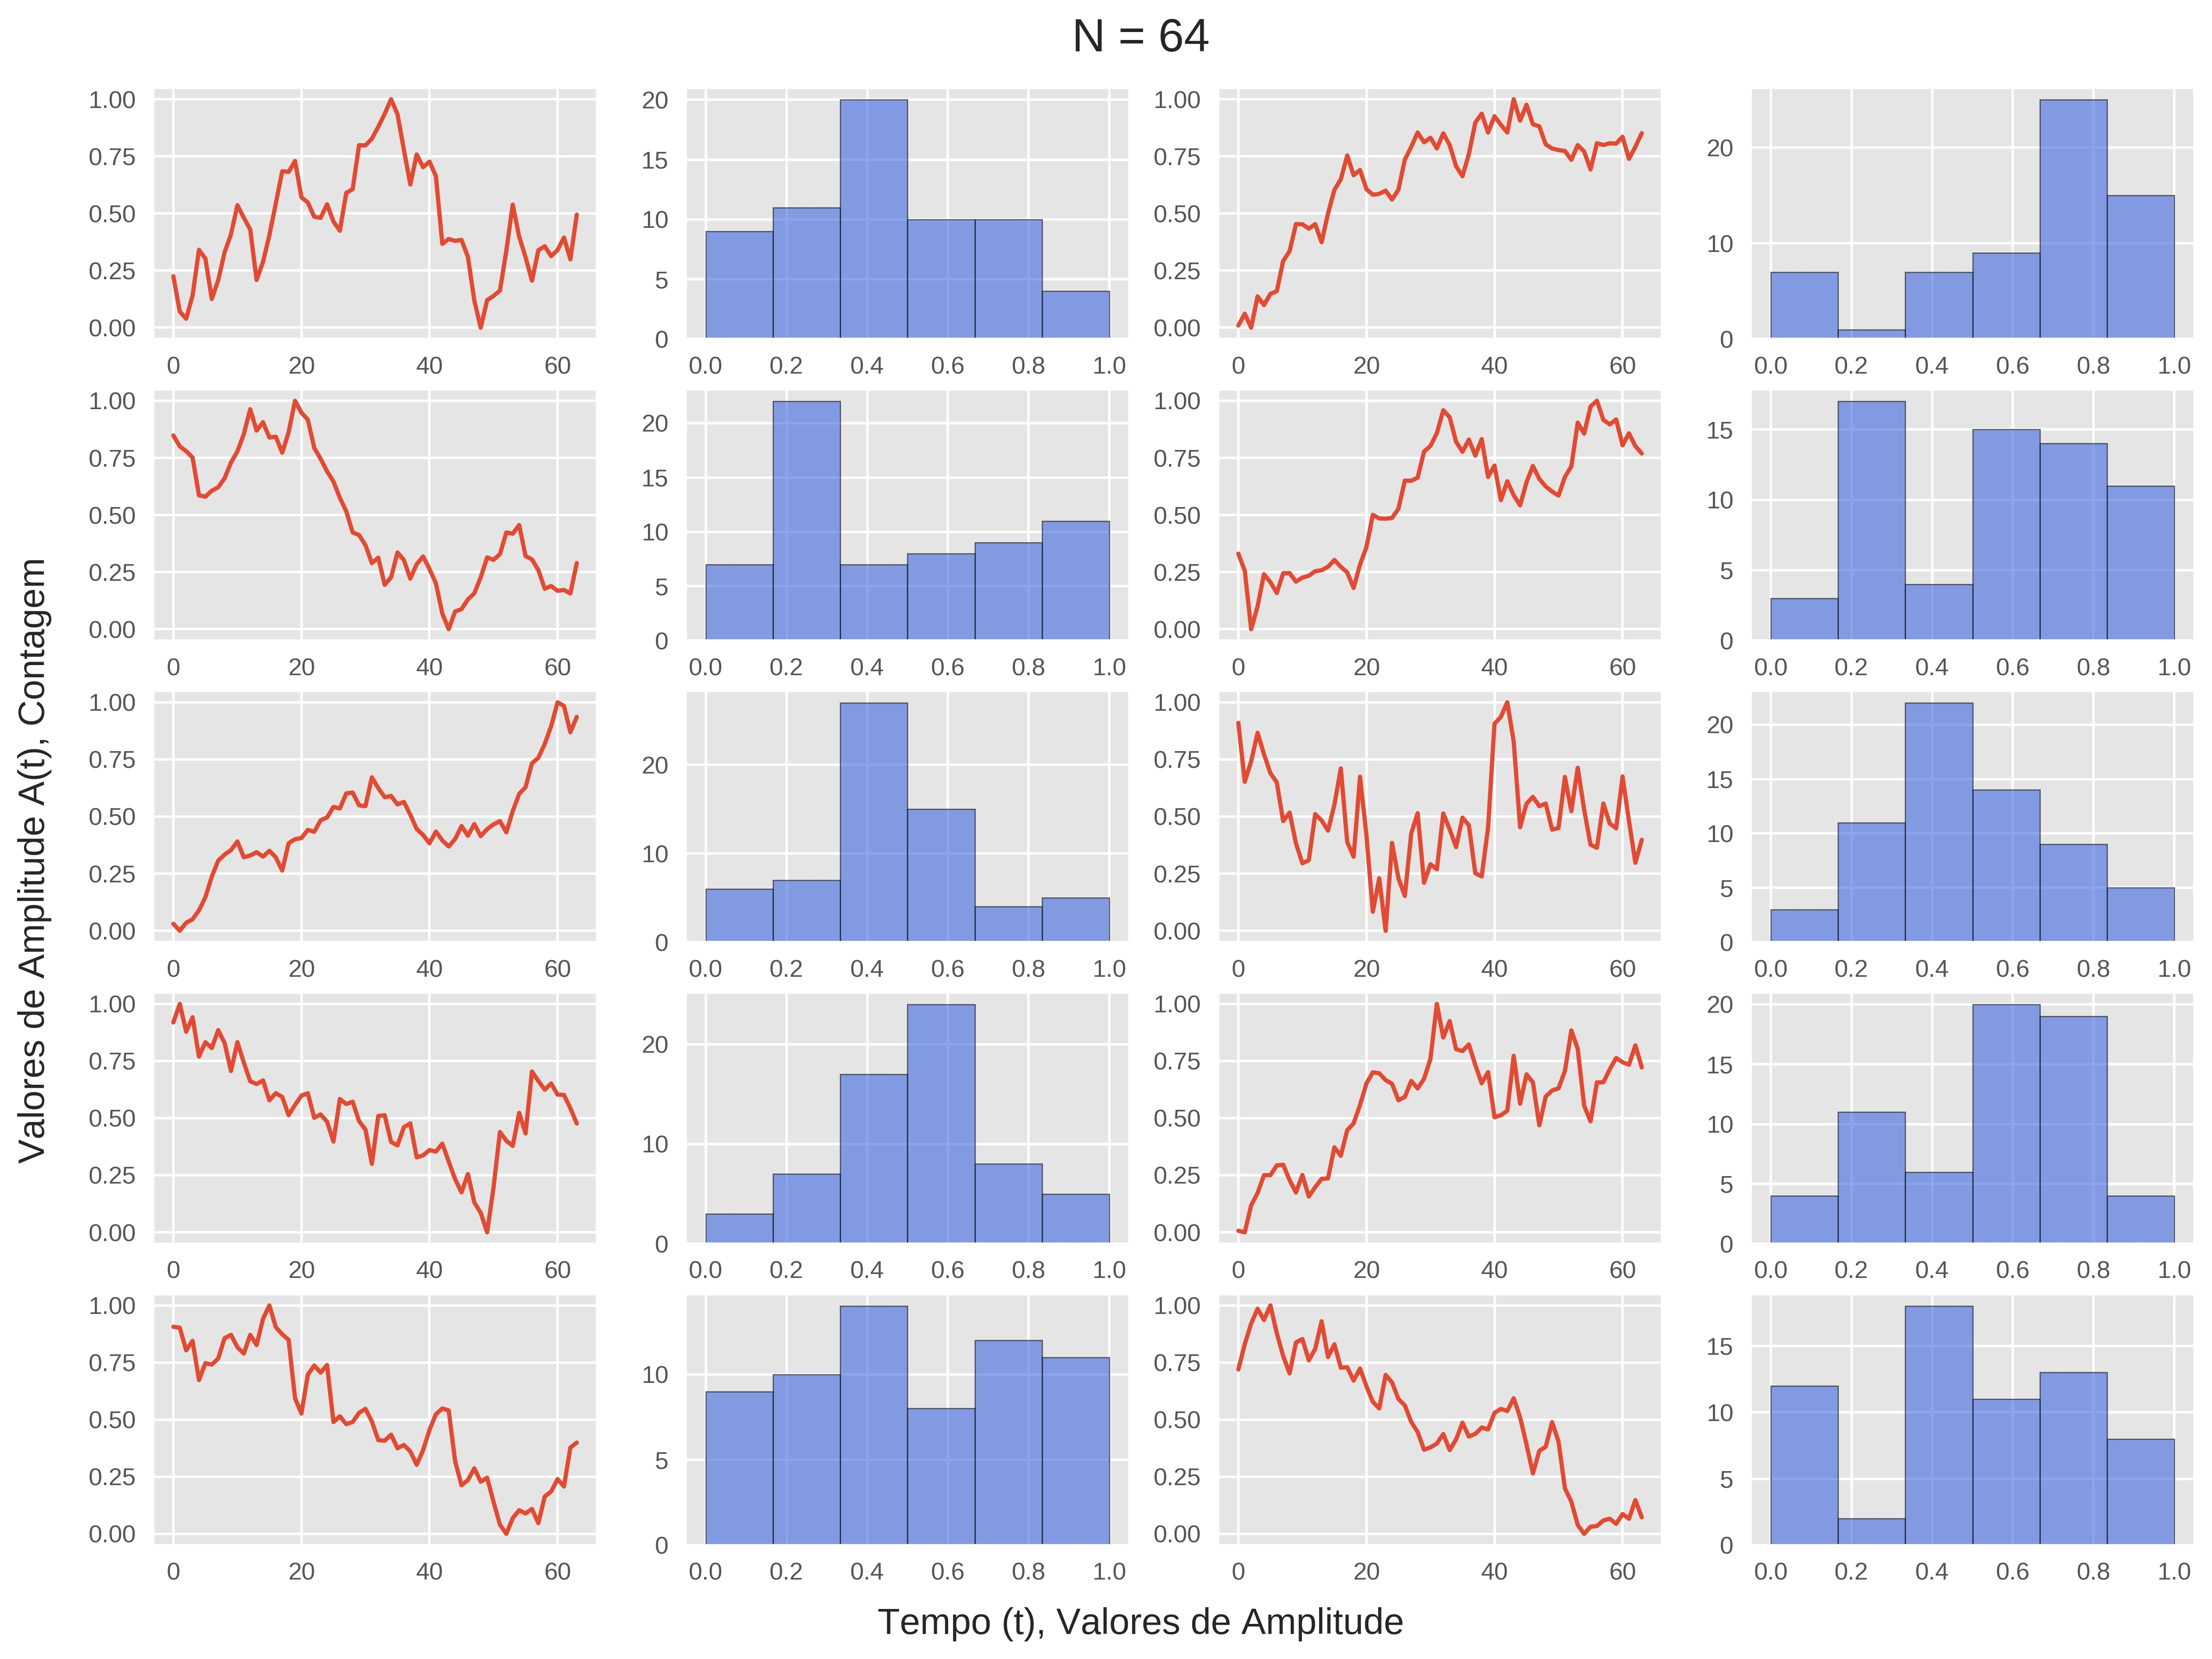
\includegraphics{Figuras/ex1/Exercicio1_n_64.jpg}}		
	\end{center}
	\vspace{-2mm}	% acrescentar o espaçamento vertical apropriado entre a borda inferior da figura e a legenda ou a fonte quando não há legenda (o valor pode ser negativo para subir)
	\legenda{Figura 1.1: Dez sinais e seus respectivos histogramas para  asérie com $N$ = 64 do grupo noise.}	% legenda - para deixar sem legenda usar comando \legenda{} (nunca deve-se comentar o comando \legenda)
	\label{ex1_fig1}
	%\FONTE{}	% fonte consultada (elemento obrigatório, mesmo que seja produção do próprio autor)
\end{figure}

Os resultados da análise foram armazenados em três arquivos .csv: \textit{Exercicio1\_momentos.csv}, contendo os quatro momentos estatísticos de cada sinal gerado, \textit{Exercicio1\_parametros.csv}, com a variância, skewness e kurtosis de todos os sinais, e \textit{Exercicio1\_kmeans.csv}, que armazena o resultado da análise dos clusters via kmeans, com as coordenadas de cada centróide gerado para cada número de cluster testado e suas respectivas inércias. Foram testados de um a oito clusters para as séries da família noise. Os plots a seguir ilustram o resultado da aplicação do algoritmo kmeans\_3D.py no espaço de parâmetros variância x skewness x kurtosis. O método do cotovelo identificou que três clusters são ideais para classificar os sinais desta família.

\begin{figure}[ht!]
	%\caption{Série e histogramas.}
	\vspace{0mm}	% acrescentar o espaçamento vertical apropriado entre o título e a borda superior da figura
	\begin{center}
		\resizebox{16cm}{!}{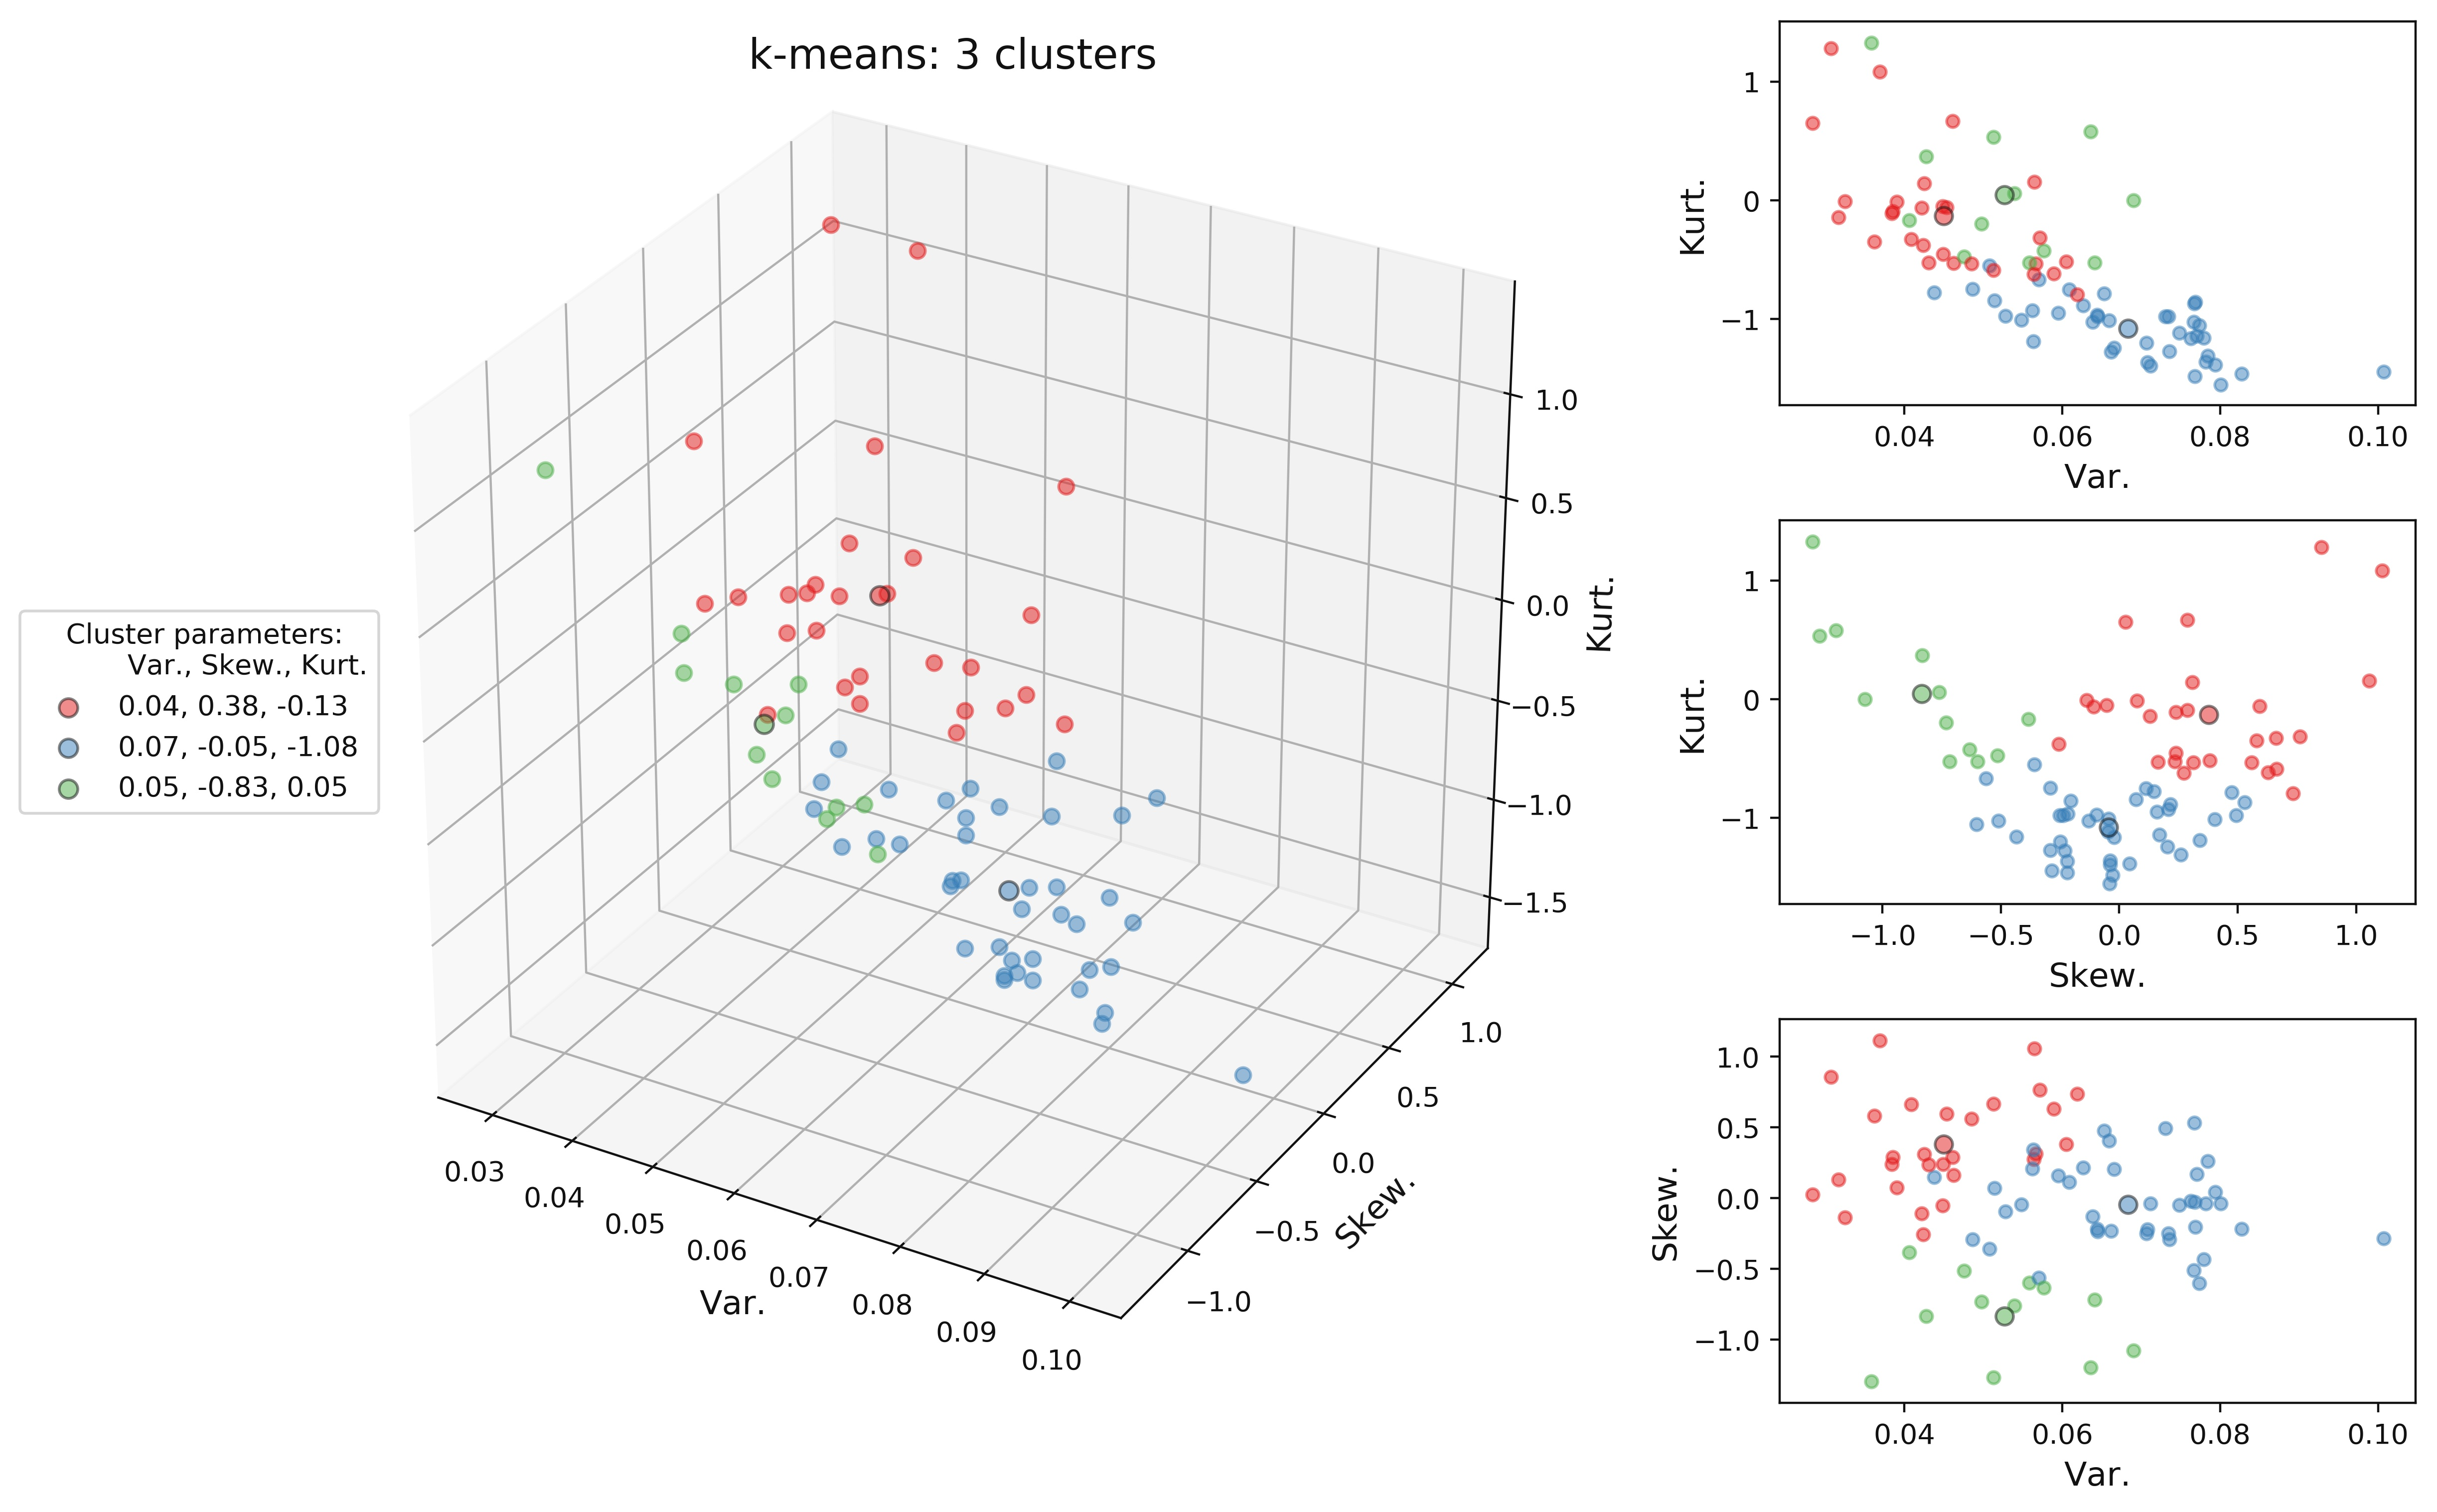
\includegraphics{Figuras/ex1/Exercicio1_cluster_3.jpg}}		
	\end{center}
	\vspace{-2mm}	% acrescentar o espaçamento vertical apropriado entre a borda inferior da figura e a legenda ou a fonte quando não há legenda (o valor pode ser negativo para subir)
	\legenda{Figura 1.2: Técnica kmeans no espaço de parâmetros variância x skewness x kurtosis para a família de sinais noise. Resultado para número de clusters $n\_c$ = 3.}	% legenda - para deixar sem legenda usar comando \legenda{} (nunca deve-se comentar o comando \legenda)
	\label{ex1_fig2}
	%\FONTE{}	% fonte consultada (elemento obrigatório, mesmo que seja produção do próprio autor)
\end{figure}

\begin{figure}[ht!]
	%\caption{Série e histogramas.}
	\vspace{0mm}	% acrescentar o espaçamento vertical apropriado entre o título e a borda superior da figura
	\begin{center}
		\resizebox{11cm}{!}{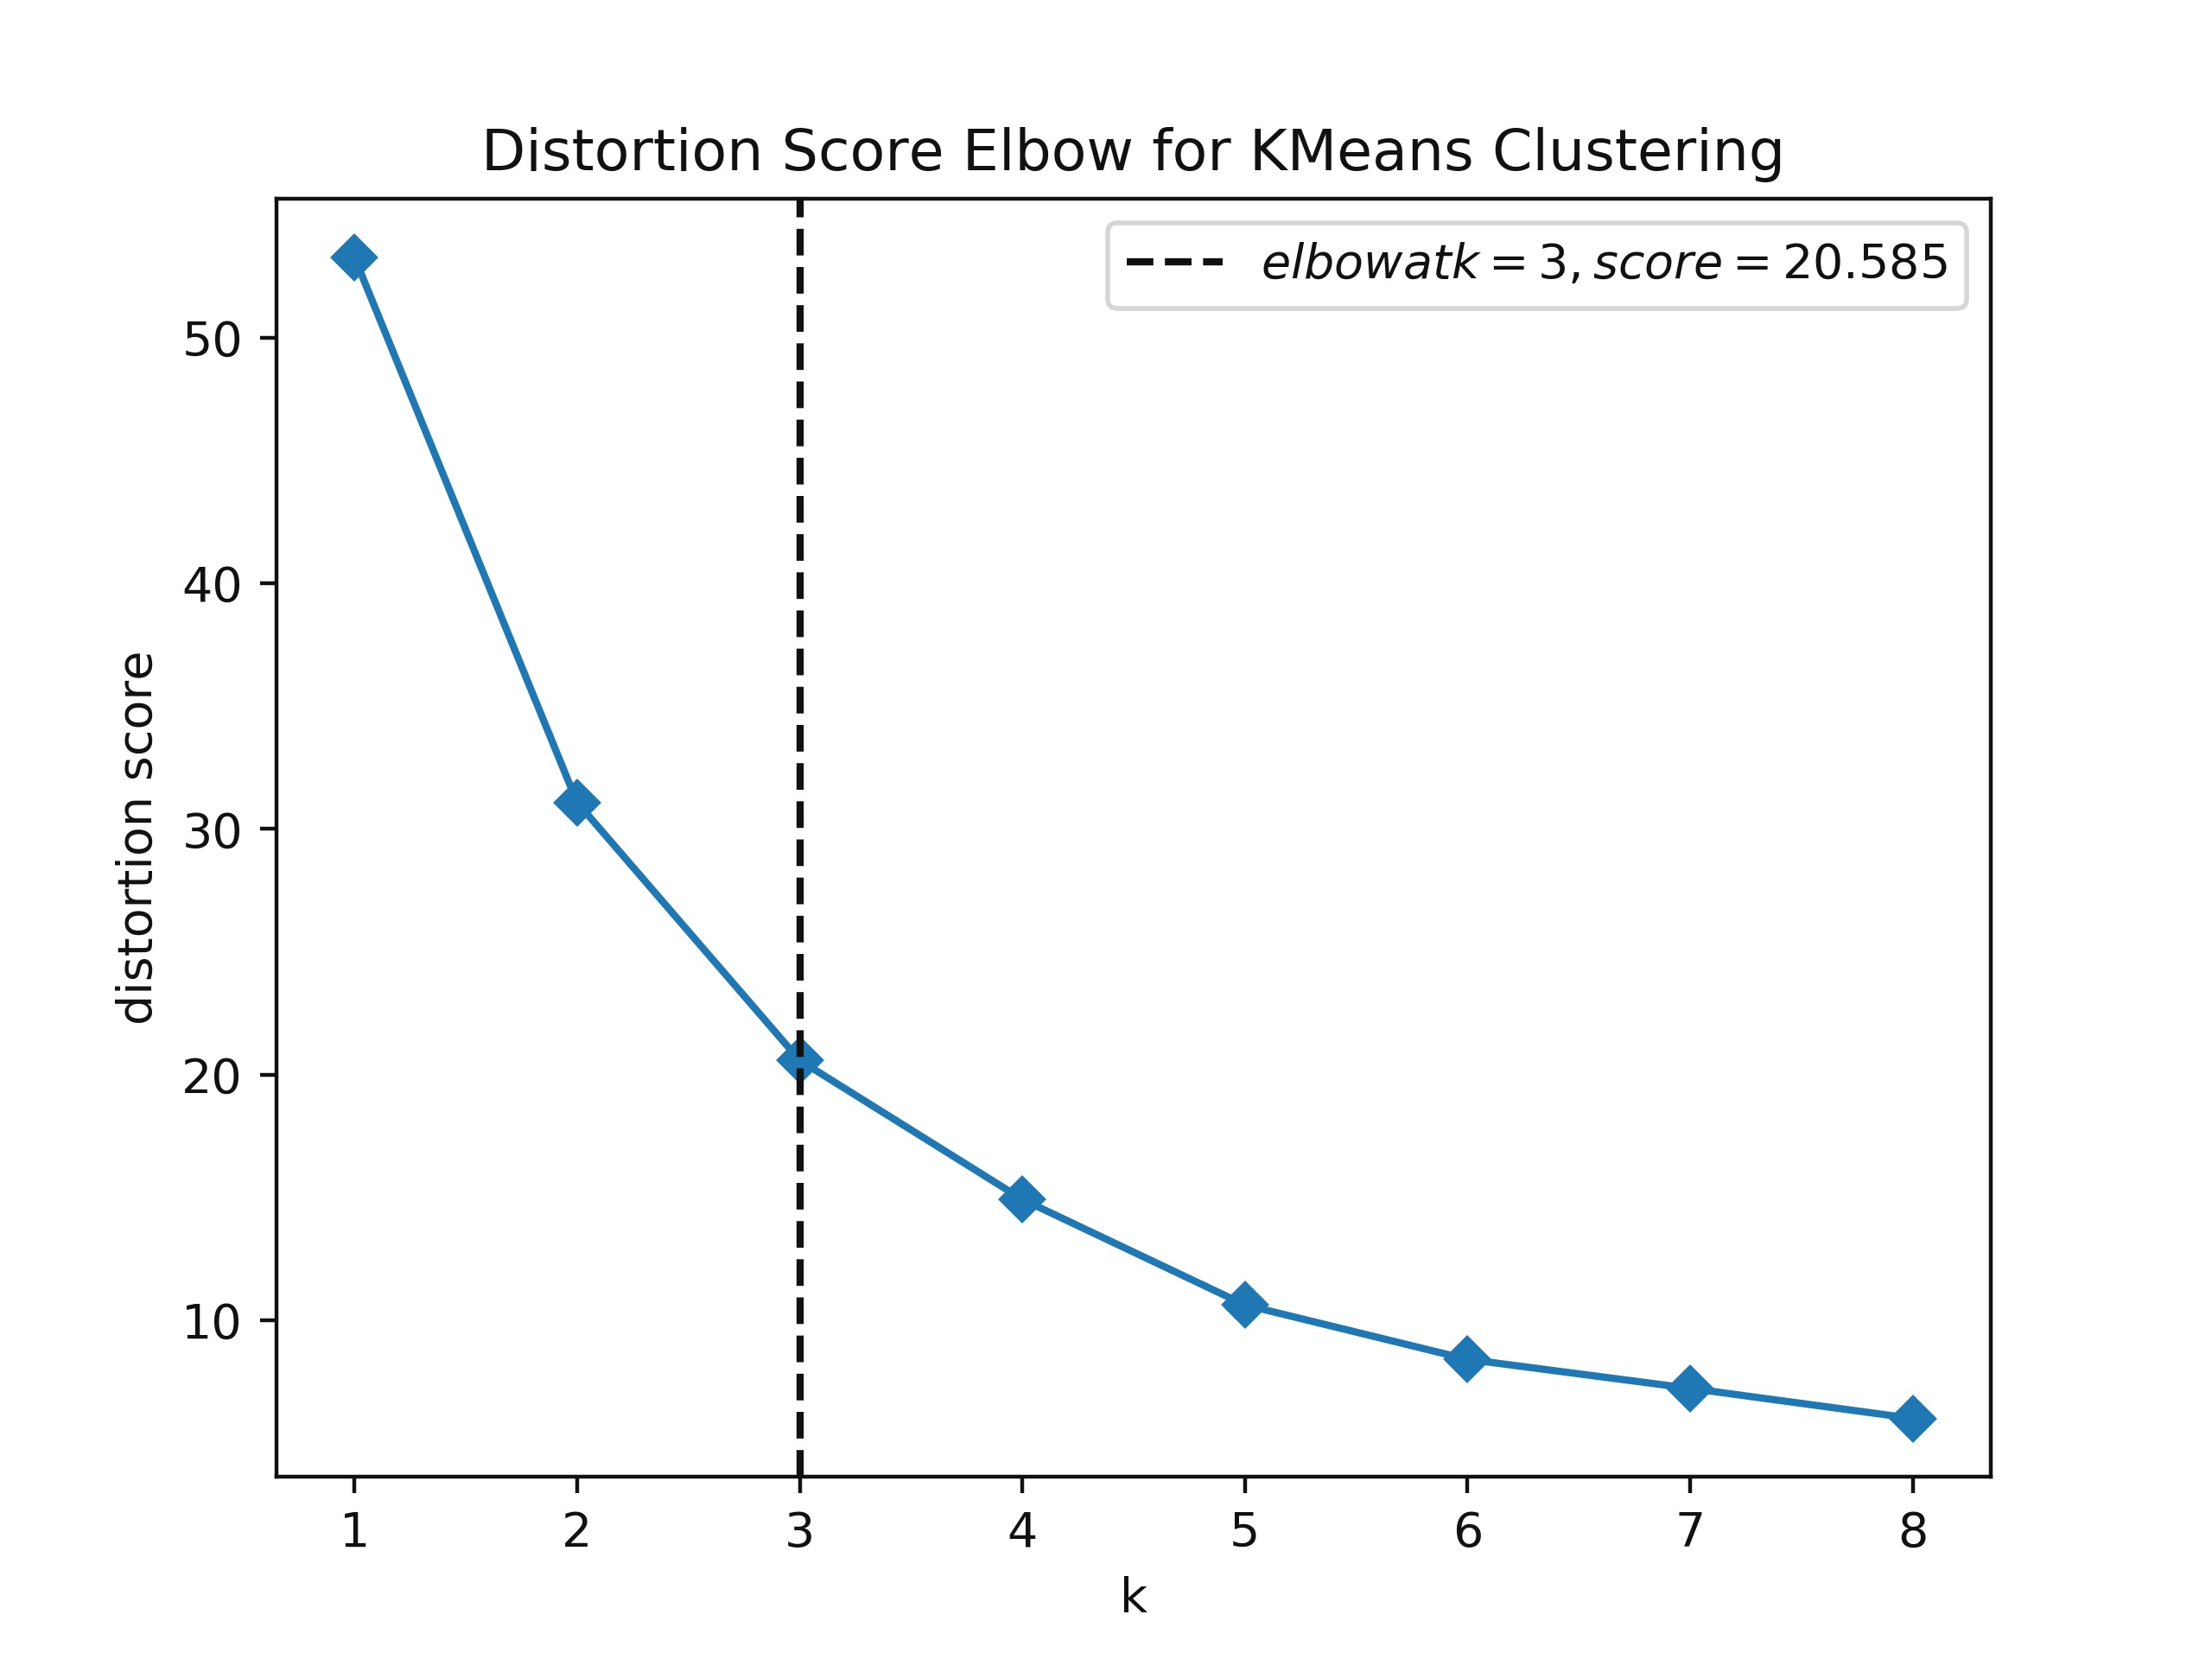
\includegraphics{Figuras/ex1/Exercicio1_elbow_algorithm.jpg}}		
	\end{center}
	\vspace{-2mm}	% acrescentar o espaçamento vertical apropriado entre a borda inferior da figura e a legenda ou a fonte quando não há legenda (o valor pode ser negativo para subir)
	\legenda{Figura 1.3: Resultado do método do cotovelo, com o gráfico de número de clusters x inércia dos centróides. O pacote yellowbric.cluster foi utilizado para determinar o número de clusters ideal.}	% legenda - para deixar sem legenda usar comando \legenda{} (nunca deve-se comentar o comando \legenda)
	\label{ex1_fig3}
	%\FONTE{}	% fonte consultada (elemento obrigatório, mesmo que seja produção do próprio autor)
\end{figure}
%
%\subsection*{1.1}
%\addcontentsline{toc}{section}{\protect\numberline{} 1.1}%

%O script \textit{noise.py}, utilizado para gerar os sinais, se encontra na pasta \textit{signal\_generator\_codes}. Ele tem como input o tamanho da série $n$. Além de gerar as séries, ele também gera o histograma e os respectivos plots, bem como arquivos \textit{momentos.csv} e \textit{parametros.csv} com os valores de todos os momentos estatísticos e parâmetros relevantes para este exercício (variância, skewness e kurtosis).

%\subsection*{1.2}
%\addcontentsline{toc}{section}{\protect\numberline{} 1.2}%

%O script de análise estatística \textit{stats\_tools.py} incorpora funções de normalização e de cálculo dos momentos estatísticos. Ele é importado a partir da pasta \textit{statistical\_analysis\_codes}.

%\subsection*{1.3}
%\addcontentsline{toc}{section}{\protect\numberline{} 1.3}%

%O script \textit{kmeans\_3D.py} analisa qualquer conjunto tridimensional de dados. Além dos dados, o número de clusters a serem testados também é um dos inputs. Ele gera gráficos dos dados no espaço de parâmetros sendo analisado, e determina o melhor número de cluster pelo método do cotovelo. O arquivo \textit{kmeans.csv} gerado pelo script contém informação das coordenadas x, y e z do centróide e da inércia para cada número de cluster testado. No presente exercício 8 clusters foram avaliados. O algoritmo \textit{kmeans\_3D.py} se encontra na pasta \textit{statistical\_analysis\_codes}.
